\chapter{Introducción}
    
        \section{\textcolor{dark_violet}{\textbf{GraviCap}}, ¿Qué es?}
            \textcolor{dark_violet}{\textbf{GraviCap}} consiste en un condensador de energía gravitatoria junto a un sistema de control de consumo.\par
            Un condensador de energía gravitatoria, o batería de gravedad es una estructura que eleva una carga consumiendo energía eléctrica, para luego almacenarla en forma de energía potencial gravitatoria. El sistema de control de consumo, revisa constantemente el consumo de energía de la red, eligiendo el momento indicado para soltar la carga, que generará la energía cinética que, luego, será transformada en energía eléctrica por un generador.\par
            \textcolor{dark_violet}{\textbf{GraviCap}}, es un prototipo que ha llevado mucho esfuerzo. Desde sus inicios con una ardua investigación hasta su construcción. Este esfuerzo no se limita solo a la construcción de un prototipo, sino que \textcolor{dark_violet}{\textbf{GraviCap}} busca generar un impacto significativo en la forma en que almacenamos energía a nivel mundial. Tal como se detalla en Alcances (\ref{Alc}), \textcolor{dark_violet}{\textbf{GraviCap}} no solo tiene el \textbf{potencial de transformar el almacenamiento de energía} en Argentina, aprovechando las condiciones geográficas favorables del país, sino también de posicionar a nuestro proyecto como una referencia en el ámbito internacional. Al adoptar un enfoque innovador y sostenible, creemos que \textcolor{dark_violet}{\textbf{GraviCap}} puede desempeñar un papel clave en la transición hacia un futuro energético más limpio y eficiente.\par

        \section{Alcances}
        \label{Alc}
            \subsection{Impacto en Argentina}
                La Argentina posee condciones geográficas muy favorables para la implementación de \textbf{energías renovables}, como la solar y la eólica, en las que \textcolor{dark_violet}{\textbf{GraviCap}} podría ser utilizado para expandir las capacidades del suministro energético argentino.\par
                Por ejemplo, \textcolor{dark_violet}{\textbf{GraviCap}} podría aprovechar zonas como:\par
                \begin{itemize} [label=•]
                    \setlength{\itemindent}{1.5em}
                    
                    \item \textbf{Cordillera de los Andes}: La región montañosa de los Andes es ideal para la instalación de baterías gravitatorias debido a su topografía pronunciada y grandes diferencias de altitud. El uso de sistemas como \textcolor{dark_violet}{\textbf{GraviCap}} en esta zona permitiría almacenar energía de manera eficiente, utilizando el desnivel natural de las montañas.\par
                    \item \textbf{Región Patagónica}: La Patagonia, conocida por sus fuertes vientos, es un punto clave para la generación de energía eólica. La instalación de \textcolor{dark_violet}{\textbf{GraviCap}} en esta región permitiría almacenar la energía producida durante los picos de viento, asegurando un suministro constante, incluso en momentos de baja producción.\par
                    \item \textbf{Noroeste Argentino}: Esta región combina un alto potencial solar y una topografía favorable con cerros y mesetas, lo que la convierte en un lugar ideal para la combinación de energía solar y almacenamiento gravitatorio. En zonas como Jujuy y Salta, la alta irradiación solar podría generar electricidad durante el día, que luego sería almacenada por \textcolor{dark_violet}{\textbf{GraviCap}} para su uso durante la noche o en días nublados.\par
                    \item \textbf{Cuyo}: Las provincias de San Juan y Mendoza, además de tener un alto potencial para la energía solar, también cuentan con relieves montañosos que permiten una fácil implementación de \textcolor{dark_violet}{\textbf{GraviCap}}. La combinación de ambos factores ofrecería una solución integrada para el almacenamiento y el aprovechamiento de energía renovable, mejorando la autosuficiencia energética de la región.\par
                \end{itemize}

            \subsection{Impacto Mundial}
                \textcolor{dark_violet}{\textbf{GraviCap}} se presenta como un innovador prototipo de batería gravitatoria, con el objetivo de posicionar a la Argentina en la vanguardia del almacenamiento de energía y las \textbf{energías renovables}. Este proyecto no solo explora una tecnología emergente, sino que también introduce una nueva corriente de pensamiento en el ámbito global, proponiendo soluciones sostenibles y eficientes frente a los desafíos energéticos contemporáneos. \textcolor{dark_violet}{\textbf{GraviCap}} busca ampliar los horizontes del almacenamiento de energía, aprovechando la fuerza de la gravedad como una fuente renovable, y apunta a generar un impacto significativo en la transición hacia sistemas energéticos más limpios y ecológicos. A través de este enfoque, se abre la posibilidad de fortalecer el rol de Argentina en la adopción de tecnologías de vanguardia, impulsando la innovación en el sector energético tanto a nivel local como internacional.\par
            \subsection{Impacto Social}
                La implementación de la tecnología de \textcolor{dark_violet}{\textbf{GraviCap}} en Argentina podría tener un profundo impacto social, al abordar varios desafíos clave relacionados con el desarrollo sostenible, la equidad energética y la creación de oportunidades económicas.\par
                \begin{enumerate}
                    \setlength{\itemindent}{2.5em}
                    
                    \item \textbf{Acceso a energía limpia y asequible}: \textcolor{dark_violet}{\textbf{GraviCap}} ofrecería una solución innovadora para el almacenamiento de energía renovable, facilitando el acceso a fuentes de energía más limpias y sostenibles. Esto contribuiría a reducir la dependencia de combustibles fósiles, lo que impactaría directamente en la disminución de la huella de carbono y en la mejora de la calidad del aire, con efectos positivos en la salud pública y el bienestar de las comunidades, especialmente en áreas rurales o con dificultades para acceder a fuentes de energía convencionales.\par
                    \item \textbf{Desarrollo económico y generación de empleo}: La fabricación, implementación y mantenimiento de esta tecnología fomentaría la creación de empleo en diversas áreas, desde la ingeniería hasta la instalación y el mantenimiento de los sistemas, generando nuevas oportunidades laborales en sectores emergentes. Además, al posicionar a Argentina como pionera en tecnologías de almacenamiento de energía gravitatoria, se abriría el camino para atraer inversiones y fomentar el desarrollo de una industria energética renovable más robusta y diversificada.\par
                    \item \textbf{Descentralización energética}: Al permitir el almacenamiento eficiente de \textbf{energías renovables}, como la eólica o la solar, \textcolor{dark_violet}{\textbf{GraviCap}} podría impulsar la creación de sistemas de energía descentralizados. Esto favorecería la autonomía energética de comunidades aisladas o con escasa infraestructura eléctrica, mejorando la calidad de vida y proporcionando a las regiones más alejadas una herramienta crucial para su desarrollo.\par
                    \item \textbf{Educación e innovación tecnológica}: La introducción de esta tecnología también incentivaría la formación de nuevas generaciones de técnicos e ingenieros especializados en \textbf{energías renovables}. Esto no solo elevaría el nivel educativo del país, sino que también fomentaría una cultura de innovación y sostenibilidad, inspirando a investigadores y emprendedores locales a explorar nuevas soluciones tecnológicas para los retos energéticos y medioambientales.\par
                    \item \textbf{Reducción de la pobreza energética}: Al facilitar un acceso más estable y accesible a fuentes de energía renovable, \textcolor{dark_violet}{\textbf{GraviCap}} podría contribuir a reducir la pobreza energética en Argentina. Esto es especialmente relevante en comunidades vulnerables, que podrían beneficiarse de un suministro energético más confiable y a costos más bajos, mejorando su calidad de vida.
                \end{enumerate}
                En resumen, \textcolor{dark_violet}{\textbf{GraviCap}} tiene el potencial de ser una herramienta transformadora no solo en términos tecnológicos, sino también en su capacidad para mejorar el bienestar social, fomentar el crecimiento económico y consolidar el papel de Argentina en la lucha global contra el cambio climático.\par
        
        \section{Beneficios}
            \textcolor{dark_violet}{\textbf{GraviCap}} es un proyecto ideado para acompañar a los distintos generadores de energías renovables, adaptándose a las dimensiones que desee utilizar su consumidor acorde a la capacidad de su red eléctrica. Procura resguardar su huella de carbono al estar conformado por piezas simples sin requerimientos técnicos en demasía. Gracias a esto, pueden estar fabricadas por materiales reutilizados, derivados de materias primas locales o biomateriales. Permite prescindir aquellos materiales que perjudican al ambiente durante su producción o con su posterior desecho, ya que no hay materiales peligrosos para proteger.\par
            Almacenar energía gravitatoria nos permite ser también sustentables, ya que depende únicamente de un peso y la altura. El almacenamiento de energía es una problemática cada vez mayor, y con un planeta con crecientes problemas ambientales surgen problemas si estos son contaminantes.\par
            
            
        \section{¿Por qué \textcolor{dark_violet}{\textbf{GraviCap}}?}
            Siempre que se presenta un producto innovador surge una problematica, ¿Por qué usarlo y no usar un método más convencional?\par
            En este caso, ¿Por qué usar \textcolor{dark_violet}{\textbf{GraviCap}} y no una batería convencional?\par
            
            \subsection{Almacenamiento de Energías Renovables}
                Con la cada vez más creciente demanda y utilización de las energías renovables, como la eólica y la solar, nos encontramos con el principal problema que conllevan. Al depender de fenómenos meteorológicos para producir energía, se vuelven impredecibles y variables, cuando la red eléctrica exige una entrega constante.\par
                Para rectificar su entrega, la solución predilecta es acompañar al generador de una batería que almacene el excedente producido en momentos de superávit energético, y entregue en los momentos de déficit.\par
                Así surge una situación compleja: ¿Cómo almacenamos energía? Se presentan dos principales escenarios:\par

                \begin{itemize} [label=•]
                    \setlength{\itemindent}{1.5em}
                        \item Almacenar de forma eficiente el exceso: Cuando las condiciones son tan favorables que se produce más de lo que se demanda.\par
                        \item Recuperar el exceso: Cuando las condiciones no son favorables, la energía producida no es suficiente para cubrir la demanda.\par
                \end{itemize}
                
            \subsection{¿Por qué es necesario?}
                 El almacenamiento de energía representa una excelente oportunidad para la integración de fuentes renovables en el sistema eléctrico. No solo implica una mejora en la flexibilidad y seguridad del sistema, sino también un aumento en su eficiencia global.\par
                 Desde la perspectiva de las empresas de servicios públicos, la estrategia de almacenamiento ofrece una manera efectiva de reducir los costos de generación eléctrica. Almacenar la electricidad durante las horas valle, es decir, durante la noche cuando la demanda es baja, y luego descargarla durante las horas punta del día, cuando la demanda alcanza su pico máximo, se traduce en beneficios sustanciales. Cuanto mayor sea la disparidad entre la demanda en las horas punta y valle, mayores serán los beneficios derivados del almacenamiento de energía.\par
                 Además de los beneficios económicos, esta práctica también conduce a una generación más uniforme de energía, lo que a su vez mejora la eficiencia general del sistema. La capacidad de suavizar las fluctuaciones en la generación de energía contribuye a una operación más estable y confiable del sistema eléctrico en su conjunto. En resumen, el almacenamiento de energía no solo ofrece ventajas económicas, sino que también promueve una operación más eficiente y sostenible del sistema eléctrico.\par
                 
            \subsection{Beneficios del almacenamiento}
                 Para el transporte y la distribución energética:\par
                    
                \begin{itemize} [label=•]
                    \setlength{\itemindent}{1.5em}
                        \item Aumentar la eficiencia de la red, cuando hay congestión en la red no hay tiempo para satisfacer la demanda y el almacenamiento ayuda a liberar esta congestión.\par
                        \item Aumentar la capacidad efectiva de transporte y distribución debido a las posibilidades de carga y descarga a alta velocidad.\par
                        \item Incrementar la capacidad de distribuir energía cerca del consumo, reduciendo las pérdidas técnicas y la congestión.\par
                \end{itemize}
                    
                 Para el consumidor:\par
                    
                \begin{itemize} [label=•]
                    \setlength{\itemindent}{1.5em}
                        \item Continuidad de suministro, si se producen fallos en las redes el almacenamiento ayudará a mantener constante el suministro.\par
                        \item Reducción de costes, las empresas eléctricas pueden fijar precios variables en el tiempo (menor precio por la noche y mayor por el día) para dar un incentivo a los consumidores; al aplanar la curva de la demanda.\par
                \end{itemize}
                    
                 Para la generación de energía:\par
                 
                 \begin{itemize} [label=•]
                    \setlength{\itemindent}{1.5em}
                        \item Incrementar la fiabilidad del sistema, cuando la generación es mediante una fuente de energía renovable, sol o viento, con el almacenamiento se asegura el suministro, aunque no brille el sol o no haya viento.\par
                        \item Arbitraje de energía en tiempo real.\par
                        \item Regulación de tensión y corriente.\par
                \end{itemize}

            \subsection{Contaminación de Baterías}
                En el panorama actual, el uso de baterías ha experimentado un crecimiento exponencial, impulsado por avances tecnológicos, la creciente demanda de dispositivos electrónicos portátiles y la transición hacia vehículos eléctricos. Este aumento en la adopción de baterías como fuente de energía móvil ha generado una preocupación creciente sobre la gestión adecuada de los residuos resultantes de su desecho.\par
                Las baterías, en su variedad de formas y tipos, contienen una combinación de elementos que pueden ser perjudiciales para el medio ambiente y la salud humana. Entre estos componentes se encuentran el mercurio (Hg), el cadmio (Cd), el plomo (Pb), el níquel (Ni), el manganeso (Mn) y el zinc (Zn), sustancias que, si no se manejan adecuadamente, pueden contaminar el suelo y el agua, y representar un riesgo para la vida silvestre y los ecosistemas.\par
                Según el tipo de electrolito que contienen, las baterías pueden ser clasificadas en secas o húmedas. Las baterías de uso doméstico típicamente tienen electrolito seco, el cual puede ser alcalino o ácido, como se detalla en la tabla \ref{tab:1}. En algunos casos particulares, el electrolito ácido puede estar contenido en un gel, el cual está cubierto por un material permeable o de fibra de vidrio para su seguridad y manejo adecuado.\par
                La duración y el tipo de manejo requerido también son factores determinantes en la clasificación de las baterías, agrupándolas en primarias o desechables, y secundarias o recargables. Por lo general, para propósitos comerciales y técnicos, las baterías son tipificadas según sus componentes, lo cual puede observarse en las tablas \ref{tab:1} y \ref{tab:2}.\par
                
                \begin{table}[!htbp]
                    \centering
                    \begin{tabular}{|c|c|}
                         \hline
                         Tipos de Pila &  Componentes Principales\\
                         \hline
                         & Zinc 17\% (Anódo) \\
                         & Dióxido de Manganeso 29\% (Cátodo) \\
                         & Carbón 7\%\\
                         Carbono-Zinc & Mercurio 0,01\% (Anódo, Cátodo y Electrolito) \\
                         (C-Zn) & Cadmio 0,08\%\\
                         & Cloruro de Amonio (Electrolito)\\
                         & Plástico y Lámina 26\%\\
                         \hline
                         & Zinc 14\% (Anódo)\\
                         & Dióxido de Manganeso 22\% (Cátodo)\\
                         & Carbón 2\%\\
                         Alcalinas & Mercurio 0,5\% a 1\% (Anódo)\\
                         & Hidróxido de Potasio (Electrolito)\\
                         & Plástico y Lámina 42\%\\
                         \hline
                         & Óxido de Mercurio (33\% Hg) (Cátodo)\\
                         Óxido de Mercurio & Zinc 11\% (Anódo)\\
                         (HgO) & Hidróxido de Potasio o Hidróxido de Sodio (Electrolito)\\
                         & Plástico y Lámina 29\%\\
                         \hline
                         & Zinc 30\% (Anódo)\\
                         & Óxigeno (Del Aire, Cátodo)\\
                         Zinc-Aire & Mercurio 1\%\\
                         (Zn-Aire) & Plata 1\%\\
                         & Plástico y Lámina 67\%\\
                         & Cloruro de Sodio o Hidróxido de Sodio (Electrolito)\\
                         \hline
                         & Zinc 10\% (Anódo)\\
                         & Óxido de Plata 27\% (Cátodo)\\
                         Óxido de Plata & Mercurio 1\%\\
                         (AgO2) & Cloruro de Sodio o Hidróxido de Sodio (Electrolito)\\
                         & Plástico y Lámina 29\%\\
                         \hline
                         & Litio 10\% a 30\%\\
                         Litio (Li) & Dióxido de Manganeso (Cátodo)\\
                         & Plástico y Lámina 29\%\\
                         \hline
                    \end{tabular}
                    \caption{Componentes principales de las pilas primarias (Desechables)}
                    \label{tab:1}
                \end{table}

                \begin{table}[!htbp]
                    \centering
                    \begin{tabular}{|c|c|}
                         \hline
                         & Cadmio (Cd) 18\%\\
                         Níquel-Cadmio (Ni-Cd) & Níquel (Ni) 20\%\\
                         & Hidróxido de Potasio o de Sodio\\
                         \hline
                         Níquel-Metal Hidruro & Níquel (Ni) 25\%\\
                         (Ni-MH) & Hidróxido de Potasio\\
                         \hline
                         & Óxido de Litio-Cobalto (Cátodo)\\
                         Ión-Litio (Ión-Li) & Carbón altamente cristalizado (Anódo)\\
                         & Solvente orgánico (Electrolito)\\
                         \hline
                         Plomo & Plomo\\
                         (Pb) & Ácido Sulfúrico\\
                         \hline
                    \end{tabular}
                    \caption{Componentes principales de las pilas secundarias (Recargables)}
                    \label{tab:2}
                \end{table}
                \newpage
                Las pilas de C-Zn, utilizadas en los dispositivos electrónicos más comunes, son propensas a quemarse por sobrecalentamiento. Una vez quemadas liberan altas cantidades de metales pesados al ambiente en una reacción exotérmica incontrolable. Existen estudios que indican que el 35\% de la contaminación de mercurio producida es a causa de la quema de baterías de C-Zn junto con la basura común.\par
                También, estudios médicos han demostrado que un alto nivel de mercurio en la sangre provoca cambios de personalidad, pérdida de visión, sordera, problemas en los riñones y pulmones. Es altamente peligroso para las mujeres embarazadas. La vía principal de exposición al mercurio elemental es por inhalación de sus vapores. Cerca del 80\% de los vapores inhalados es absorbida por los tejidos pulmonares. Este vapor también penetra con facilidad la barrera de sangre del cerebro y su neurotoxicidad está bien documentada.\par
                La absorción intestinal de mercurio elemental es baja. El mercurio elemental puede oxidarse en los tejidos corporales a la forma divalente inorgánica.\par
                Se han observado trastornos neurológicos y de comportamiento en seres humanos tras inhalación de vapor de mercurio elemental. Algunos de los síntomas son: temblores, labilidad emocional, insomnio, pérdida de la memoria, cambios en el sistema neuromuscular y dolores de cabeza. Se han observado asimismo efectos en el riñón y la tiroides. Las exposiciones altas también han ocasionado mortalidad.\par
                La mayoría de las pilas y baterías recargables, actualmente carecen de mercurio.\par
                Sin embargo contienen hasta un 15\% níquel y cadmio, dos metales pesados tóxicos. El cadmio emitido al ambiente se disuelve parcialmente en el agua pero no se degrada, por lo que las plantas y animales asimilan este metal, permaneciendo en el organismo durante largo tiempo.\par
                El cadmio es calificado como cancerígeno, causante de trastornos en el aparato digestivo, produce lesiones en los pulmones. Al ingerirse se acumula en los riñones. El efecto adverso más común de exposición al níquel es una reacción alérgica, algunas personas podrían sufrir ataques de asma luego de períodos de exposición. Ciertos compuestos del níquel son posiblemente carcinógenos para los seres humanos, La exposición a niveles de manganeso muy altos durante largo tiempo ocasiona perturbaciones mentales y emocionales, y provoca movimientos lentos y faltos de coordinación.\par
                Dado que el mayor volumen consumido de pilas son alcalinas y de carbón-zinc (aproximadamente el 76\% del consumo total), el óxido de manganeso contenido en ellas es el contaminante que en mayor volumen se ha liberado al medio ambiente.\par
                Las pilas tardan más de 1000 años en degradarse, sus componentes son altamente contaminantes y no se degradan, pueden empezar a separarse luego de 50 años al aire libre. Los metales de mayor preocupación, presentes en las pilas de uso doméstico son el Hg, Cd, Mn, Ni, y Zn.\par 
                Aunque el litio en sí mismo no es considerado como un contaminante, es importante tener en cuenta que muchos de los componentes empleados en las baterías que contienen litio pueden ser altamente perjudiciales para el medio ambiente y la salud humana. Por ejemplo, el cobalto, un metal comúnmente utilizado en este tipo de baterías, es altamente tóxico. La exposición al cobalto puede provocar una serie de efectos adversos para la salud, como vómitos, náuseas, problemas de visión, trastornos cardíacos y daños en la tiroides. Esta información destaca la importancia de no solo considerar el impacto ambiental directo de las baterías, sino también los efectos secundarios asociados con los materiales utilizados en su fabricación.\par
                            
        \section{Estado del Arte}
            Actualmente, en el ámbito global, existe únicamente una empresa que se dedica a la construcción de Baterías de Gravedad conocida como \href{https://www.energyvault.com}{Energy Vault} con sede en Suiza. La empresa ha logrado construir baterías en el mundo como \href{https://www.energyvault.com/projects/zhangye}{una batería en China} o \href{https://www.renewableenergyworld.com/storage/energy-vault-lands-partnership-for-building-based-gravity-storage/}{un proyecto en Australia}.\par
            \begin{figure} [ht]
                \centering
                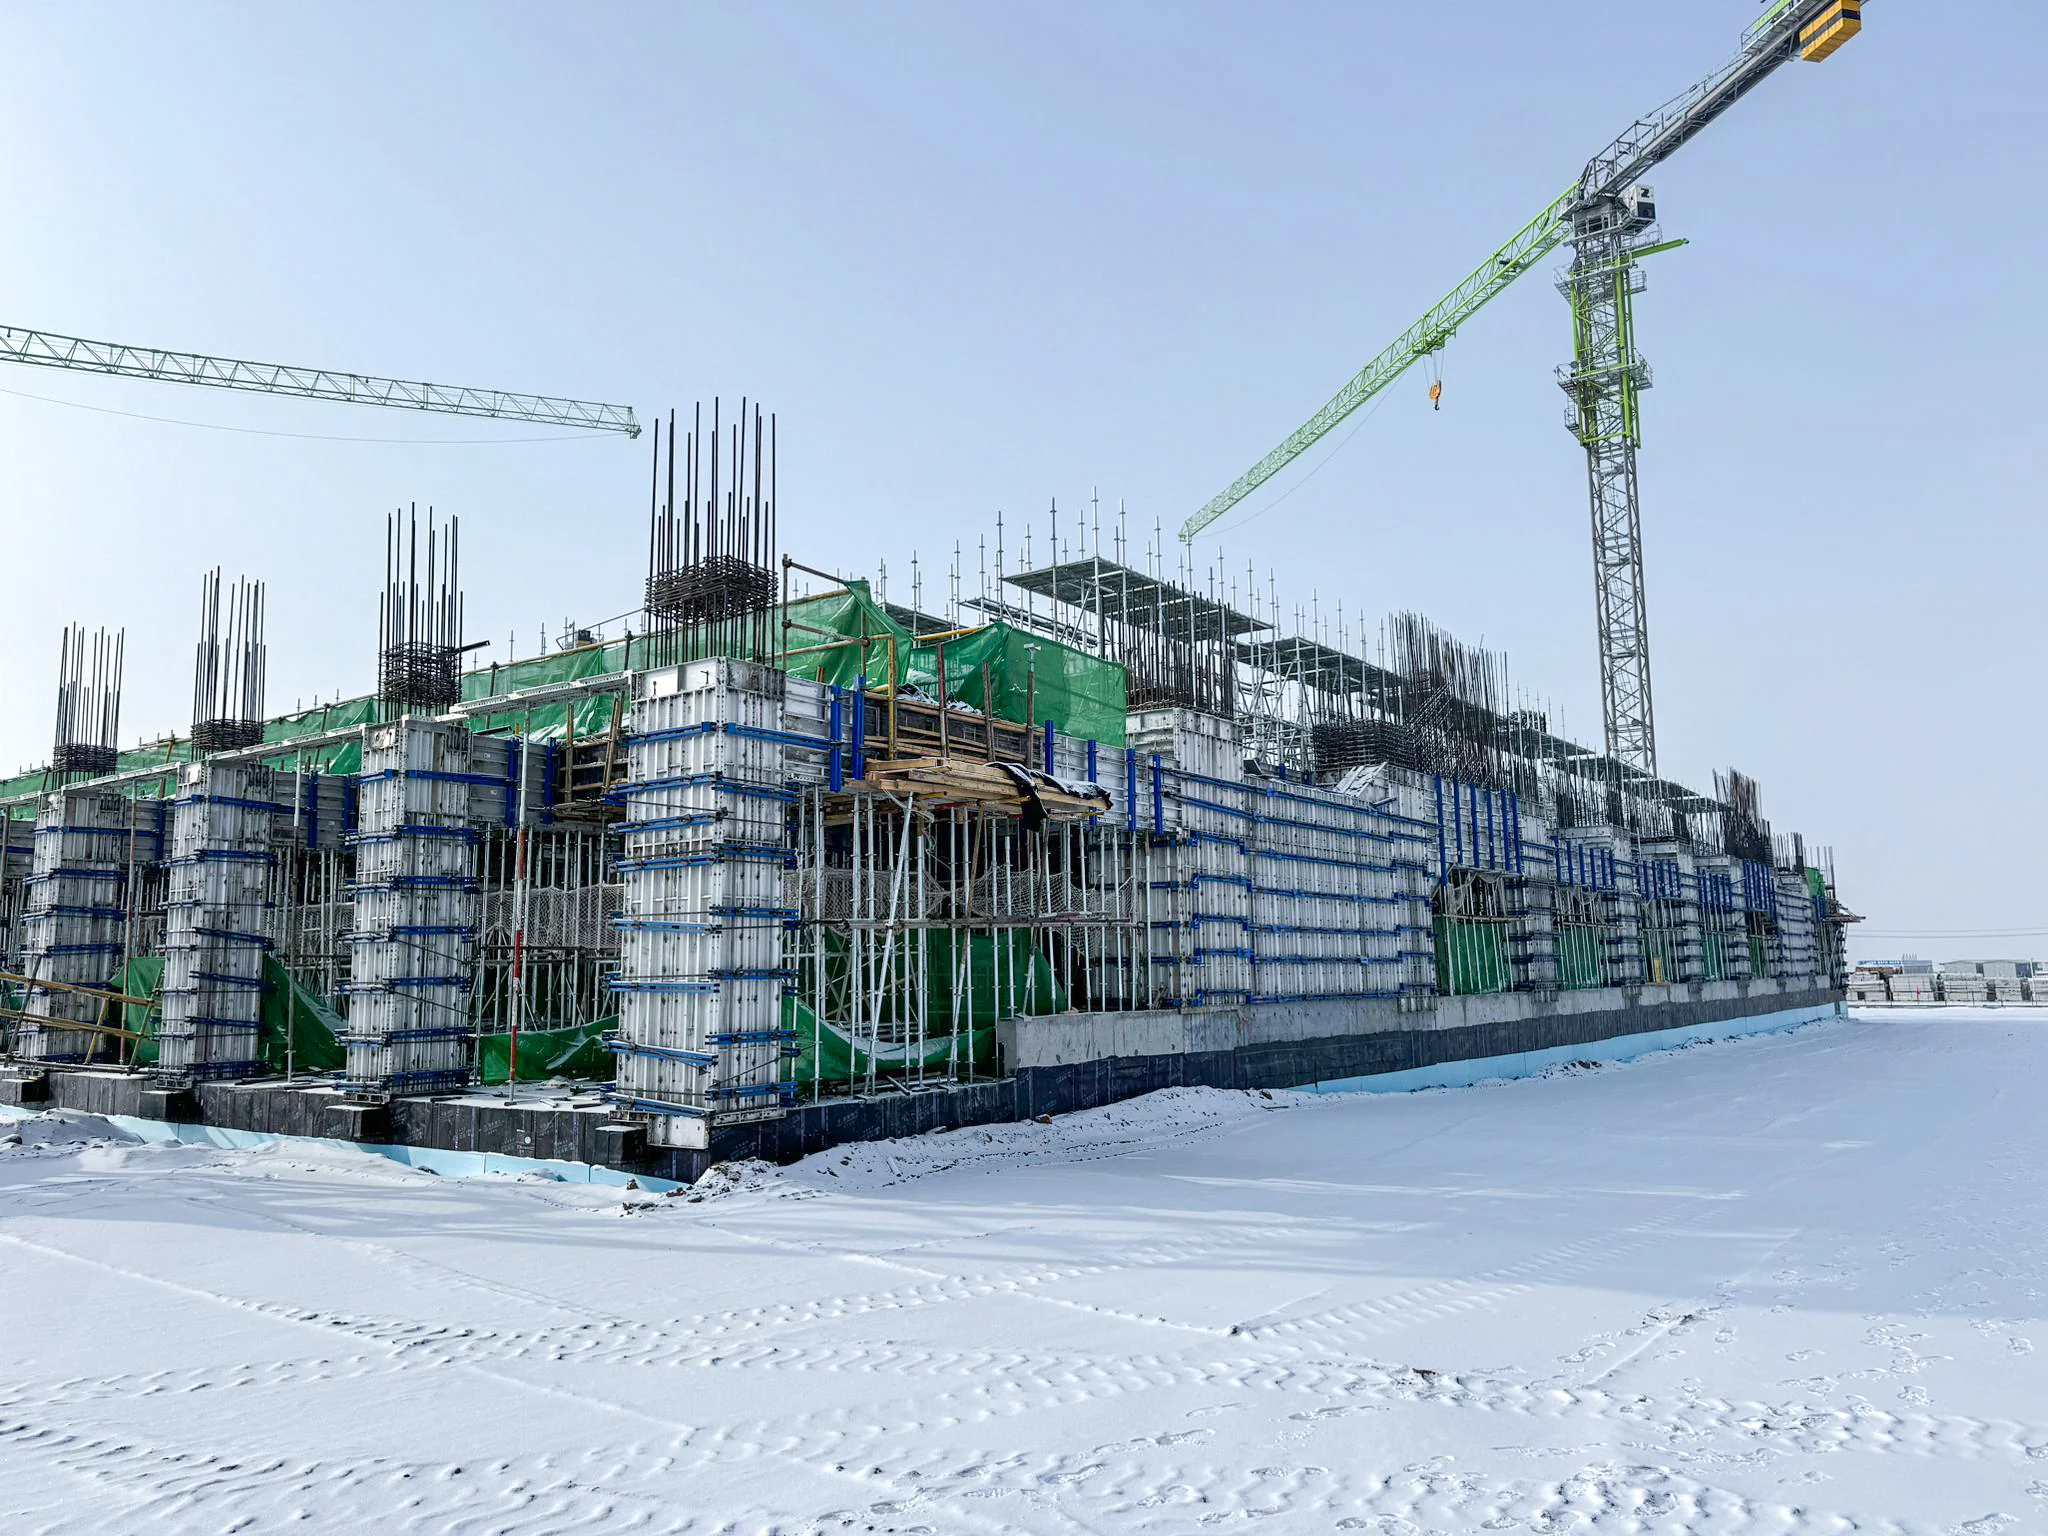
\includegraphics [width=10cm]{Introducción/Zhangye.png}
                \caption{Proyecto de Construcción en Zhangye, China}
                \label{fig:Zhangye}
            \end{figure}
            Energy Vault no se dedica a la comercialización directa de estas, sino que se construyen a pedido del usuario.\par
            En \textcolor{dark_violet}{GraviCap}, nuestro enfoque es totalmente opuesto. Nos esforzamos por empoderar al usuario brindándole el conocimiento necesario para construir su propio sistema y proporcionándole una guía detallada sobre los materiales adecuados para llevar a cabo el proyecto.\par

        \section{Implementación}
            La implementación de este tipo de tecnología en un inicio puede parecer costosa, pero los beneficios a largo plazo son indudables. La introducción de esta propuesta al mercado argentino, como se ha detallado en muchas ocasiones a lo largo de los textos anteriores, no solo tiene el potencial de posicionar a Argentina como un referente en el campo del almacenamiento de energías renovables, sino también de fortalecer su autosuficiencia energética. Al adoptar soluciones como \textcolor{dark_violet}{\textbf{GraviCap}}, se estaría optimizando la capacidad del país para aprovechar sus recursos naturales, como la energía solar y eólica, y al mismo tiempo, reducir la dependencia de fuentes de energía no renovables y contaminantes.\par
        
        \section{Usuarios}
            \textcolor{dark_violet}{\textbf{GraviCap}} presenta tres enfoques principales (que también llamamos \textcolor{light_violet}{\textbf{\textit{3C}}}) al futuro usuario del sistema:\par
            \begin{enumerate}
                \setlength{\itemindent}{2.5em}
                
                \item \textbf{Conocimiento}.
                \item \textbf{Concientización}.
                \item \textbf{Capacitación}.
            \end{enumerate}
            \subsection{Conocimiento}
                Este enfoque se centra en ofrecer al usuario una comprensión sólida sobre el funcionamiento de \textcolor{dark_violet}{\textbf{GraviCap}} y su papel dentro del sistema energético. El conocimiento abarca no solo los aspectos técnicos, como el proceso de conversión de energía gravitatoria a energía eléctrica, sino también los beneficios medioambientales que ofrece el uso de esta tecnología. Los usuarios serán informados sobre el impacto positivo de \textcolor{dark_violet}{\textbf{GraviCap}} en la reducción de emisiones de carbono, su eficiencia energética y su papel dentro de un sistema más amplio de energías renovables. La difusión de este conocimiento es clave para que los usuarios adopten la tecnología con confianza y se sientan parte de la transición hacia una energía más limpia y sostenible.
            \subsection{Concientización}
                \textcolor{dark_violet}{\textbf{GraviCap}} no solo busca ofrecer una solución tecnológica, sino también crear conciencia sobre la importancia de la sostenibilidad y el uso responsable de los recursos energéticos. Este enfoque busca sensibilizar a los usuarios sobre el impacto ambiental del consumo energético tradicional y cómo el uso de tecnologías limpias, como \textcolor{dark_violet}{\textbf{GraviCap}}, puede ayudar a mitigar los efectos del cambio climático. Se pondrá énfasis en la reducción de la dependencia de combustibles fósiles y en la necesidad de transitar hacia un sistema energético más equilibrado y respetuoso con el medio ambiente. La concientización también incluye la adopción de hábitos energéticos más responsables, fomentando una cultura de ahorro y eficiencia en el uso de la energía.\par
            \subsection{Capacitación}
                \textcolor{dark_violet}{\textbf{GraviCap}} ofrece a sus usuarios la oportunidad de capacitarse en el uso y mantenimiento del sistema. Este enfoque busca no solo que los usuarios comprendan cómo funciona la tecnología, sino también que adquieran las habilidades necesarias para operarla de manera autónoma y eficiente. La capacitación incluirá formación en el montaje, manejo y control de la batería gravitatoria. Además, se proporcionarán guías para el mantenimiento preventivo, asegurando la durabilidad y el buen funcionamiento del sistema a largo plazo. La capacitación también incluye un componente educativo que fomenta el conocimiento sobre energías renovables y su integración en la vida cotidiana.\par